\section{Numerical Tests}\label{se:NumericalTests}

In this section we present the numerical results obtained with the PD-ARS schemes provided in this paper.
The tests in Section \ref{se: Accuracy Tests} are designed to compare the accuracy of the schemes in various regimes.
The test in Section \ref{se: Neutrino Stationary State Test} demonstrates the realizability-preserving of PD-ARSs scheme.
All the tests in this subsection were applied with third-order accurate spatial discretization (polynomials of degree $k=2$) and time step $\dt = 0.1 \times \dx $.
\subsection{Accuracy Tests}
\label{se: Accuracy Tests}
To compare the accuracy of the IMEX scheme, we applied our PDARSs and Pareschi \& Russo \cite{pareschiRusso_2005} (SSP2332) scheme to some smooth problems in streaming, absorption, ans scattering dominated regimes in one spatial dimension.
All the tests in this subsection were applied with the maximum entropy closure in the low occupancy limit.
In the streaming test, the second-order and third-order accurate explicit strong stability-preserving Runge-Kutta methods\cite{gottlieb_etal_2001} , (SSPRK2 and SSPRK3, respectively) are also applied to serve as an reference.
More information and the definition of the absolute error and the relative error can be found in \cite{chu_2018}.

\subsubsection{Sine Wave Streaming}
This test involves the streaming part only: the collision term is turned off. 
A periodic domain $D$ was applied and the initial condition is given by...
More information can be found in \cite{chu_2018}.
In Figure ~\ref{fig: SineWaveStreaming}, the absolute error for the number density is plotted versus the number of elements $N$.
Errors obtained with SSPRK3 and PD-ARS with SSPRK3 decrease as $N^{-3}$ as expected.
All the other schemes have errors decreases as $N^{-2}$.
In the streaming limit, PD-ARSs degenerate to their explicit part, SSPRK2 and SSPRK3, respectively.
Hence, errors of PD-ARS and SSPRKs are indistinguishable on the plot.
Among the second-order schemes, SSP2332 has the smallest error.
\begin{figure}[h]
  \centering
    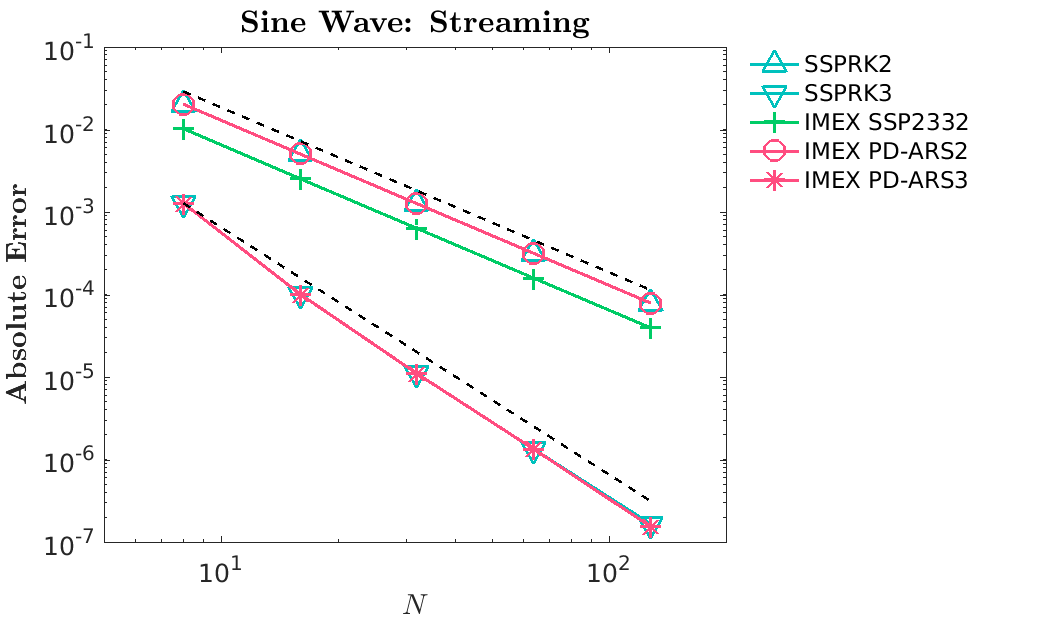
\includegraphics[width=0.6\textwidth]{figures/SineWaveStreaming}
   \caption{Absolute error versus number of elements $N$ for the streaming sine wave test.  Results employing various time stepping schemes are compared: SSPRK2 (cyan triangles pointing up), SSPRK3 (cyan triangles pointing down), SSP2332 (green crossing), PD-ARS with SSPRK2 (light red circles) and PD-ARS with SSPRK2 (light red hexagram). Black dash-dot reference lines are proportional to $N^{-1}$ (top), $N^{-2}$ (middle), and $N^{-3}$ (bottom), respectively.}
   \label{fig: SineWaveStreaming}
\end{figure}

\subsubsection{Sine Wave Damping}
Figure~\ref{fig:SineWaveDamping} shows the numerical result of sine wave damping test.
See \cite{chu_2018} for more information about the test setting.
SSP2332 as a second-order scheme display second order convergence rate.
PD-ARSs convergent in first order, as a price paid for realizability-preserving.
\begin{figure}[h]
  \centering
    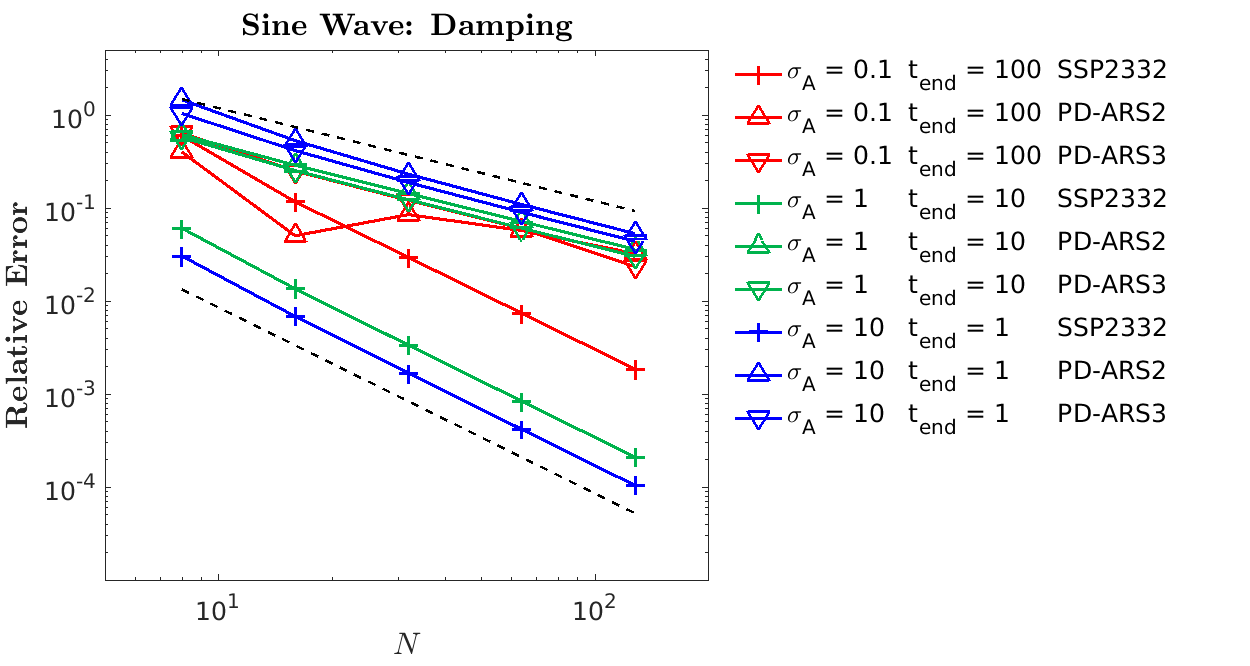
\includegraphics[width=0.7\textwidth]{figures/SineWaveDamping}
   \caption{Relative error versus number of elements $N$ for the damping sine wave test. Results for different values of the absorption opacity $\sigma_{\Ab}$, employing various IMEX time stepping schemes, are compared.  Errors for $\sigma_{\Ab}=0.1$, $1$, and $10$ are plotted with red, green, and blue lines, respectively.  The IMEX schemes employed are SSP2332 ($+$), PD-ARS with SSPRK2 (circles) and PD-ARS with SSPRK3 (hexagram).  Black dash-dot reference lines are proportional to $N^{-1}$ (top) and $N^{-2}$ (bottom), respectively.}
  \label{fig:SineWaveDamping}
\end{figure}

\subsubsection{Sine Wave Diffusion}
The last test with known smooth solution is sine wave diffusion test.
See \cite{chu_2018} for more information about the test setting.
Figure~\ref{fig:SineWaveDiffusionJ} shows the numerical result.
SSP2332 and PD-ARSs display third-order accuracy for the number density $\cJ$ and second-oder accuracy for $\cH_{x}$ and their errors are difficult to distinguish.
PD-ARS with SSP2332 behaviors as good as SSP2332 in the diffusion region but requires 1/3 less implicit solver.
\begin{figure}[h]
  \centering
  \begin{tabular}{cc}
    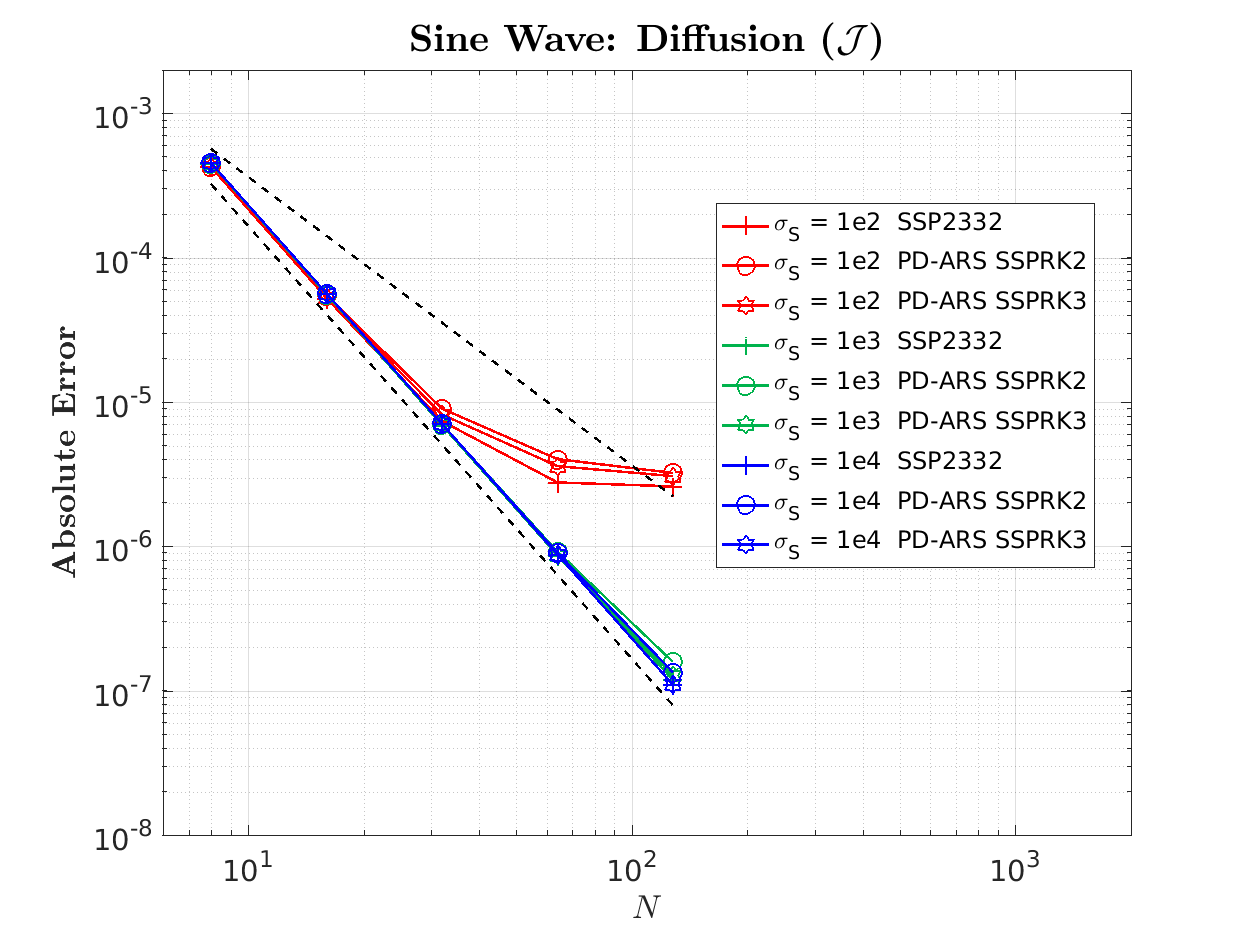
\includegraphics[width=0.5\textwidth]{figures/SineWaveDiffusionJ}
    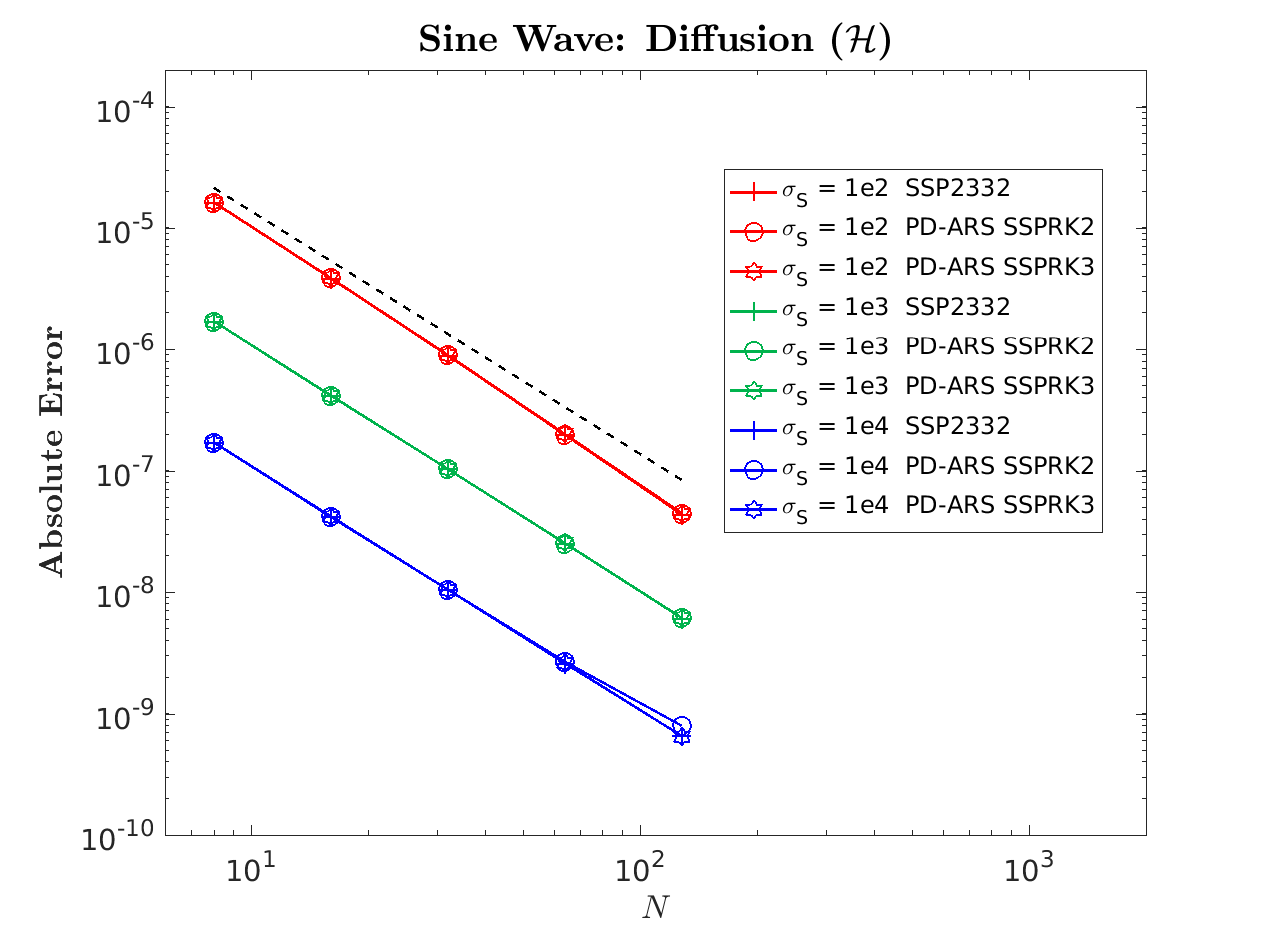
\includegraphics[width=0.5\textwidth]{figures/SineWaveDiffusionH}
  \end{tabular}
   \caption{Absolute error for the number density $\cJ$ (left) and the number flux $\cH_{x}$ (right) versus number of elements for the sine wave diffusion test.  Results with different values of the scattering opacity $\sigma_{\Scatt}$, employing different IMEX schemes, are compared.  Errors with $\sigma_{\Scatt}=10^{2}$, $10^{3}$, and $10^{4}$ are plotted with red, green, and blue lines, respectively.  The IMEX schemes employed are:  SSP2332 ($+$), PD-ARS with SSPRK2 (circles) and PD-ARS with SSPRK3 (hexagram). Black dash-dot on the left plot reference lines are proportional to $N^{-1}$ (top) and $N^{-2}$ (bottom), respectively. Black dash-dot on the right plot reference lines are proportional to $N^{-2}$ .}
   \label{fig:SineWaveDiffusionJ}
\end{figure}

\subsection{Neutrino Stationary State Test} \label{se: Neutrino Stationary State Test}
Next we consider a more realistic-like test: two-dimensional neutrino transport with emission, absorption and elastic scattering under a stationary realistic-like background.
This test is designed to test the realizability-preserving properties of the PD-ARSs schemes.
Figure~\ref{fig:NeutrinoStationaryTestEOS} plots the thermal state and the opacities we used.
This test is computed on a two-dimensional domain $D=\{\vect{x}\in\bbR^{2}:x^{1}\in[0,200], x^{2}\in[0,200]\}$ with a grid of 128 elements on each direction.
We take 10 energy groups vary from 0~MeV to 300~MeV and initial the neutrino number density $\cJ$ and flux density $\bcH$ both zero(arbitrary small).
For realizability-preserving test, CB closure with PD-ARSs schemes, SSP2332, scheme proposed by Cavaglieri \& Bewley \cite{cavaglieriBewley2015} and scheme proposed by McClarren et al. \cite{mcclarren_etal_2008} are all applied.
Only PD-ARSs schemes produces realizability-preserving result and evolve the model to a stable state.
The realizability-preserving plot and the evolve process of PD-ARSs are given in Figure~\ref{fig:NeutrinoStationaryTestEvolve}. 

\begin{figure}[h]
  \centering
  \begin{tabular}{cc}
    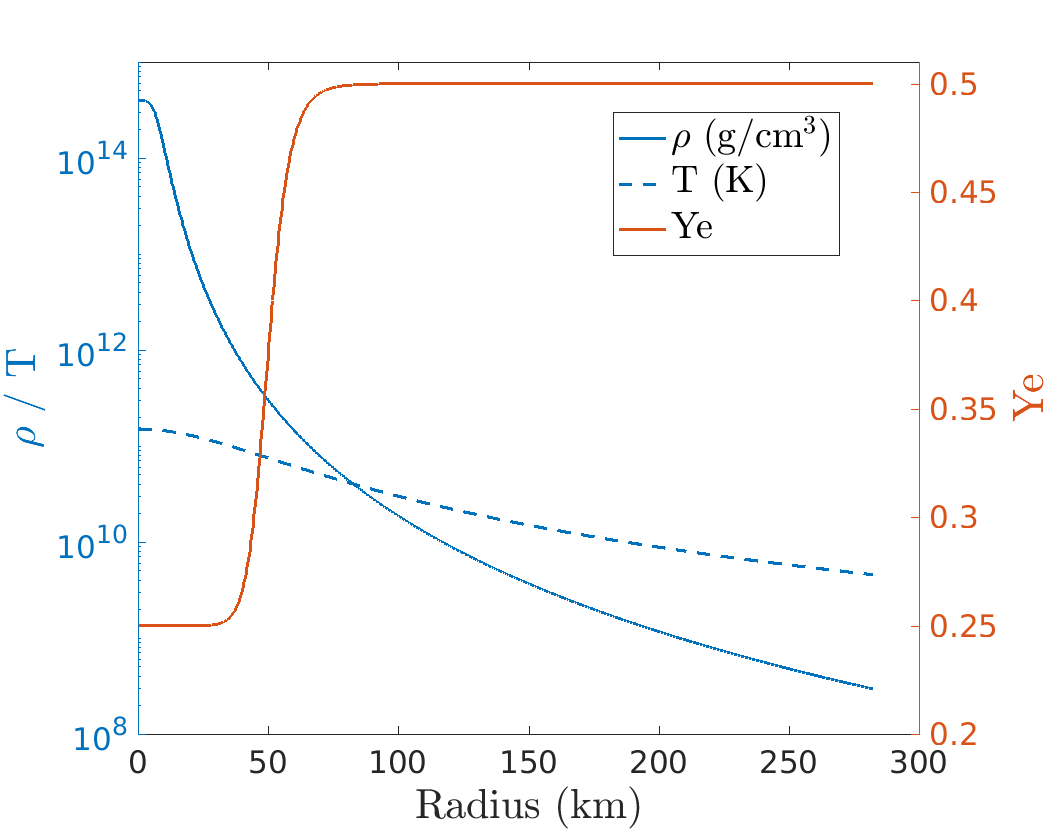
\includegraphics[width=0.45\textwidth]{figures/NStatinaryS_EOS}
    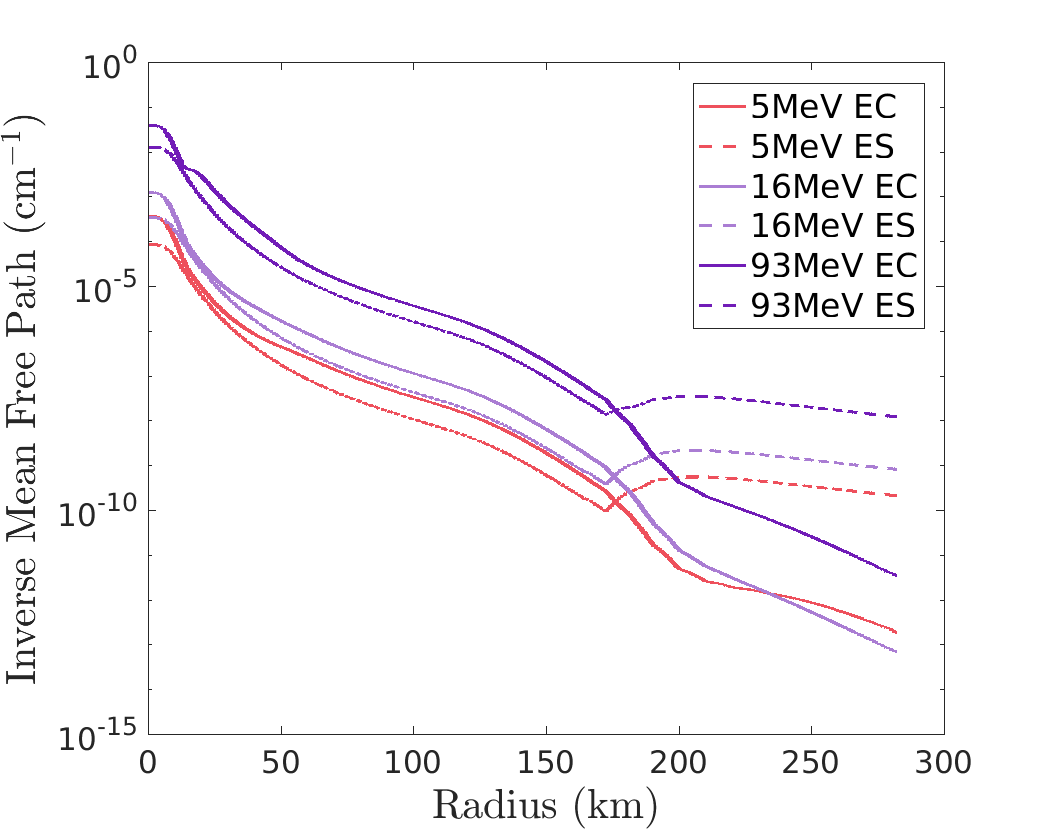
\includegraphics[width=0.45\textwidth]{figures/NSS_Opacities}
  \end{tabular}
   \caption{Thermal state plot (left) and neutrino absorptivity ($\chi$) and neutrino elastic scattering opacity ($\sigma$) in space (right) for the neutrino stationary state test.}
   \label{fig:NeutrinoStationaryTestEOS}
\end{figure}

\begin{figure}[h]
  \centering
    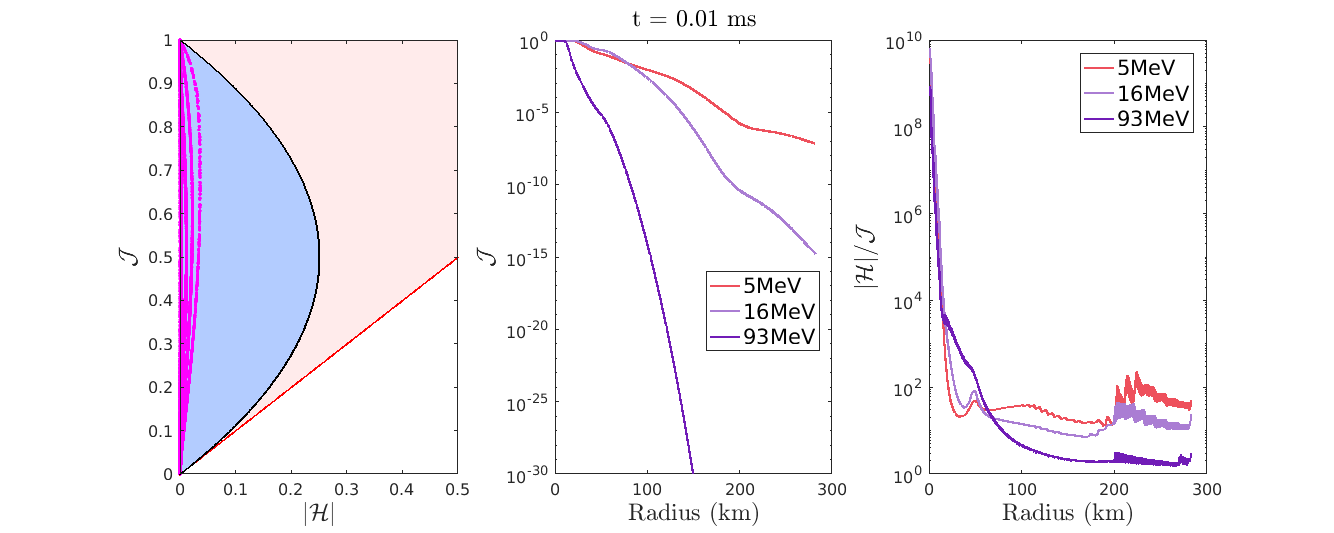
\includegraphics[width=\textwidth]{figures/NSS_1_1}\\
    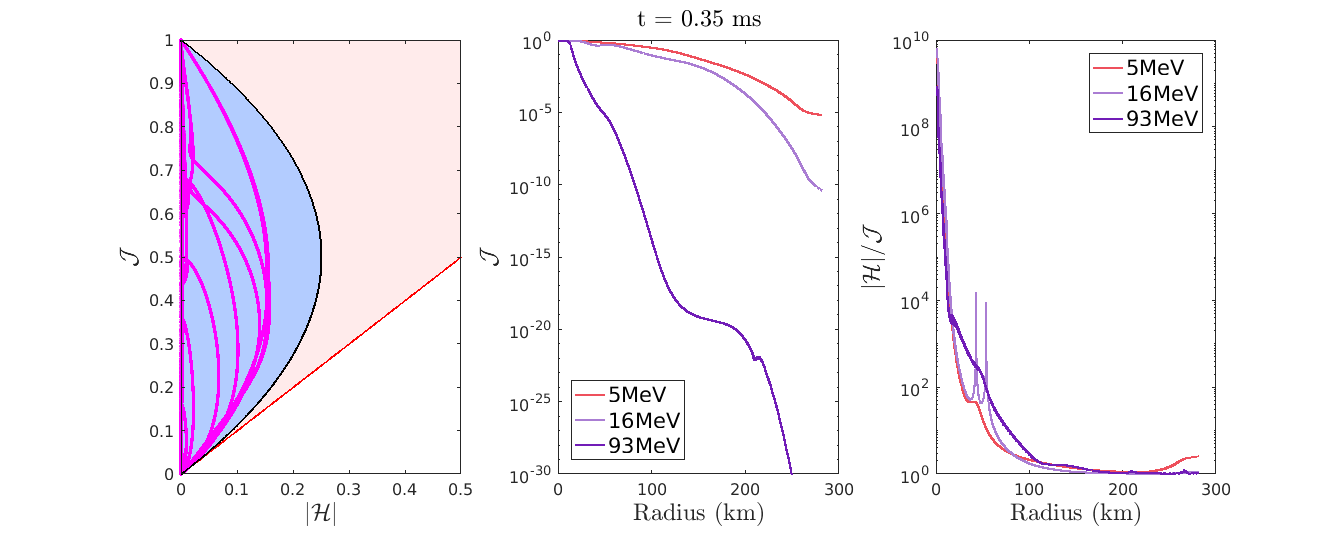
\includegraphics[width=\textwidth]{figures/NSS_3_1} \\
    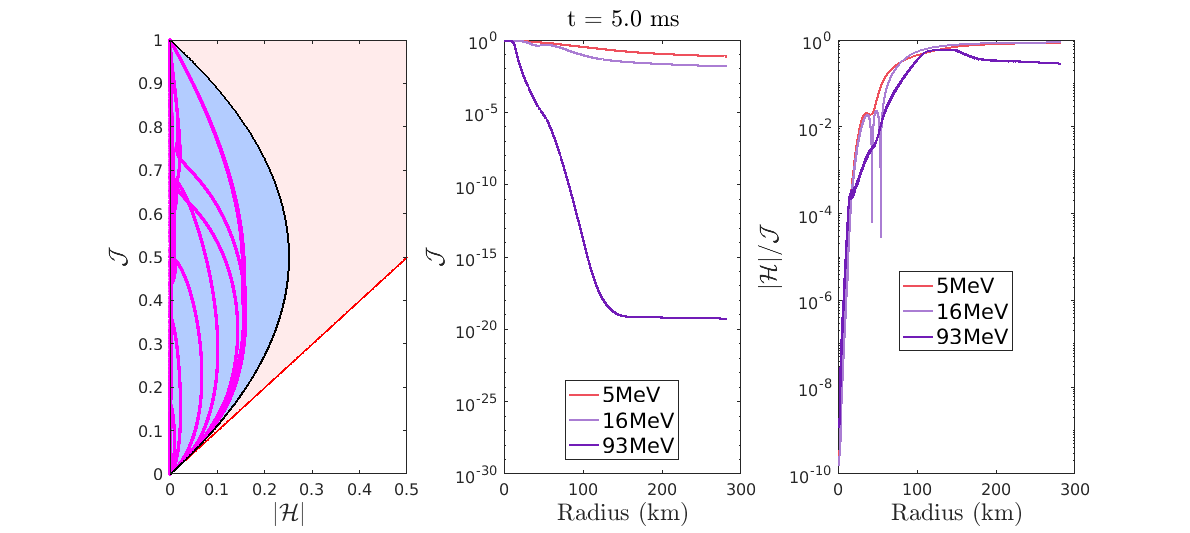
\includegraphics[width=\textwidth]{figures/NSS_5_1} \\
   \caption{Readability plots (left column), the number density $\cJ$ versus radius plots (center column) and the flux factor $|\bcH|/\cJ$ versus radius plots (right column) at t = 0.01~ms ,0.35~ms and 5.0~ms for the neutrino stationary state test. For the realizability plots, the light blue area demonstrate the realizability domain and the black lines define its boundary. Each $\bcM=(\cJ,\bcH)^{T}$ state is marked by a red dot. The results of PD-ARS with SSPRK2 and PD-ARS with SSPRK3 are indistinguishable in these plot.}
      \label{fig:NeutrinoStationaryTestEvolve}
\end{figure}